\chapter{RF PCB Design}
    \section{RF Principle}
        \begin{figure}[h]
            \centering
            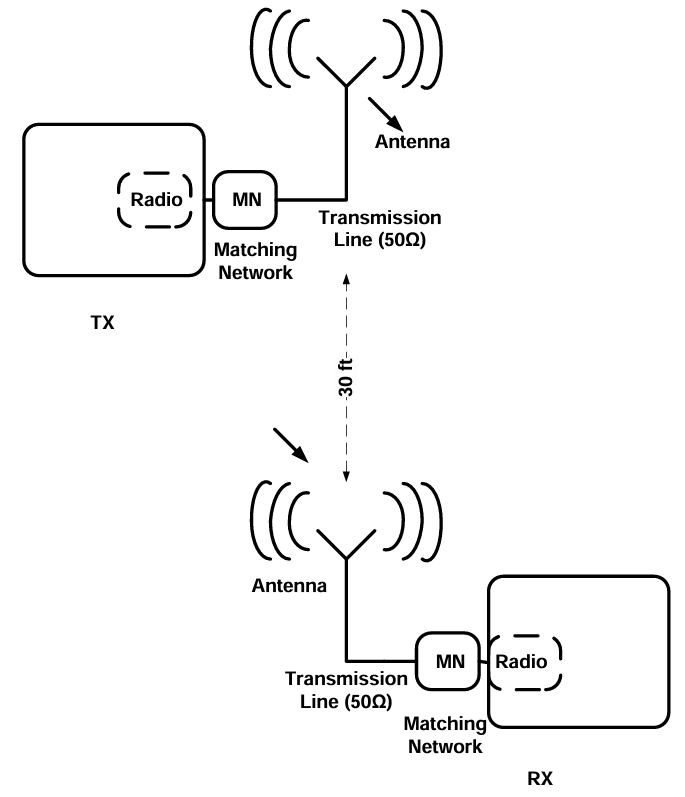
\includegraphics[width=0.5\textwidth]{figures/wireless_system.png}
            \caption{Typical Short-Range Wireless System}
            \label{fig:wireless_system}
        \end{figure}
        \newpage

        Về cơ bản, antenna là một dây dẫn lộ ra ngoài không gian. Nếu một dây dẫn có một tỉ lệ nhất định,
        hoặc là bội số bước sóng của tín hiệu\footnote{Harmonic antenna operation}, dây dẫn đó sẽ trở thành một antenna.
        Đây là điều kiện \textit{cộng hưởng}, vì năng lượng điện cung cấp cho antenna được bức xạ vào không gian.\cite{Infineon2023_rflayout}\par
        \begin{figure}[h]
            \centering
            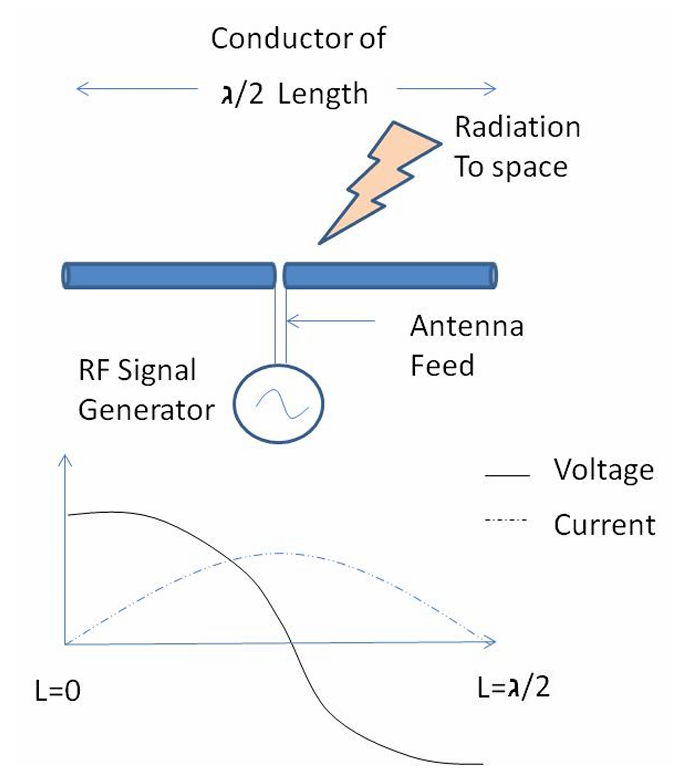
\includegraphics[width=0.5\textwidth]{figures/dipole_antenna_basic.png}
            \caption{Dipole Antenna Basic}
            \label{fig:dipole_antenna_basic}
        \end{figure}

        Trong \autoref{fig:dipole_antenna_basic}, dây dẫn có độ dài $\frac{\lambda}{2}$,
        trong đó $\lambda$ là bước sóng của tín hiệu điện.
        Nguồn phát tín hiệu cung cấp cho antenna tại điểm trung tâm
        bằng một transmission line, gọi là \textit{antenna feed}.
        Ở chiều dài này, sóng dừng điện áp và dòng điện hình thành
        trên toàn bộ chiều dài dây dẫn.\par

        \begin{figure}[h]
            \centering
            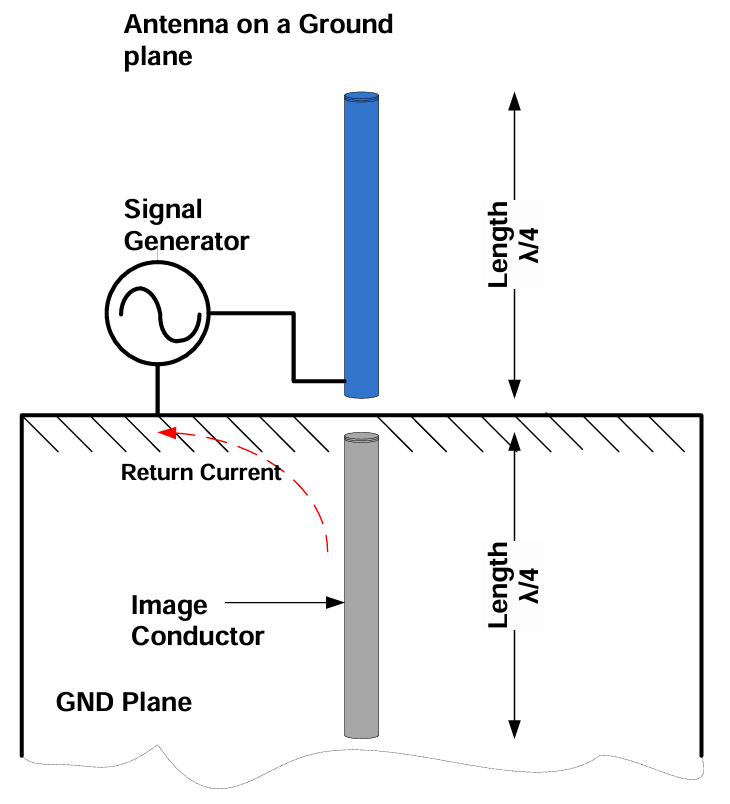
\includegraphics[width=0.35\textwidth]{figures/quarter_wave_antanna.png}
            \caption{Quarter-Wave Antenna}
            \label{fig:quarter_wave_antanna}
        \end{figure}

        Trong PCB, các mạch antenna có thể đạt được hiệu suất tương tự
        bằng cách thiết dây dẫn có chiều dài $\frac{\lambda}{4}$ bằng cách cụ thể như \autoref{fig:quarter_wave_antanna}.\par

        Bằng cách tạo ra một GND plan ở một khoảng cách nhất định bên dưới dây dẫn,
        một hình ảnh phản chiếu được tạo ra có cùng độ dài $\frac{\lambda}{4}$,
        khi kết hợp lại, nó hoạt động giống như một antenna lưỡng cực.
        Thiết kế antenna này được gọi là \textbf{quarter-wave monopole antenna} (antenna đơn cực một phần tư bước sóng).
        Tín hiệu được truyền trên một đường dẫn single-ended và GND plan hoạt động như một đường hồi tiếp.\par
    
    \section{Các loại antenna}
        \subsection{Wire antenna}
        \subsection{PCB antenna}
        \subsection{Chip antenna}

    \section{Thông số antenna}
        \subsection{Return Loss}
            \begin{equation}
                \text{Return Loss (dB)} = 10\log\left(\frac{P_{incident}}{P_{reflected}}\right)
            \end{equation}    

            \begin{figure}[h]
                \centering
                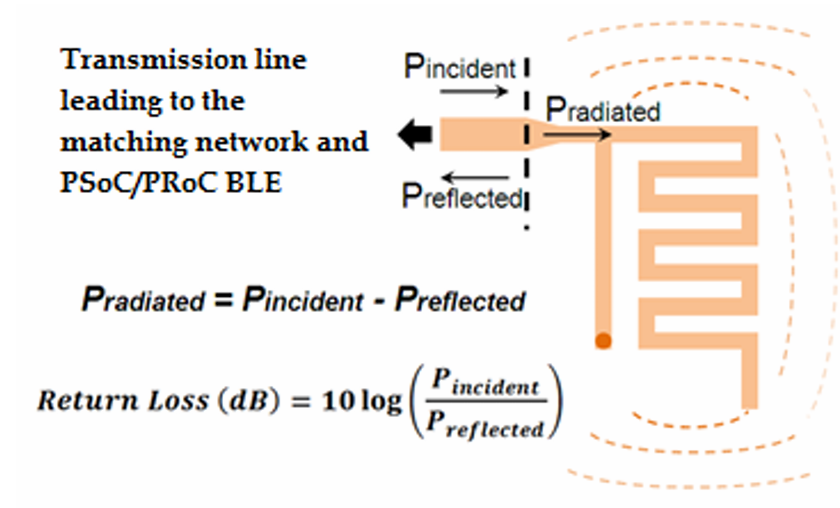
\includegraphics[width=0.5\textwidth]{figures/return_loss_antenna.png}
                \caption{Return Loss}
                \label{fig:return_loss_antenna}
            \end{figure}

            \begin{table}[h]
                \centering
                \begin{tabular}{|c|c|c|c|}
                    \hline
                    \rowcolor{TLgreen!50}
                    &   &   &   \\
                    \arrayrulecolor{TLgreen!50}
                    \cline{1-4}
                    \arrayrulecolor{black}
                    \multirow{-2}{*}{\cellcolor{TLgreen!50}$\mathbf{S_{11}}$}  &   \multirow{-2}{*}{\cellcolor{TLgreen!50}\textbf{Return Loss (dB)}}  &   \multirow{-2}{*}{\cellcolor{TLgreen!50}\textbf{$\mathbf{\frac{P_{reflected}}{P_{incident}}}$ (\%)}}    &   \multirow{-2}{*}{\cellcolor{TLgreen!50}\textbf{$\mathbf{\frac{P_{radiated}}{P_{incident}}}$ (\%)}} \\\hline
                    -20 &   20 &   1\%  &   99\% \\\hline
                    -10 &   10 &   10\% &   90\% \\\hline
                    -3  &   3  &   50\% &   50\% \\\hline
                    -1  &   1  &   79\% &   21\% \\\hline
                \end{tabular}
                \caption{Return Loss and Power Reflected from Antenna}
                \label{tab:return_loss_antenna}
            \end{table}

        \subsection{Bandwidth (Băng thông)}
            Băng thông biểu thị sự đáp ứng tần số của antenna.
            Nó biểu thị mức độ phù hợp của antenna với transmission line trên toàn bộ băng tần
            đang khảo sát, giữa 2.40 GHz và 2.48 GHz cho các ứng dụng BLE.\par

            \begin{figure}[h]
                \centering
                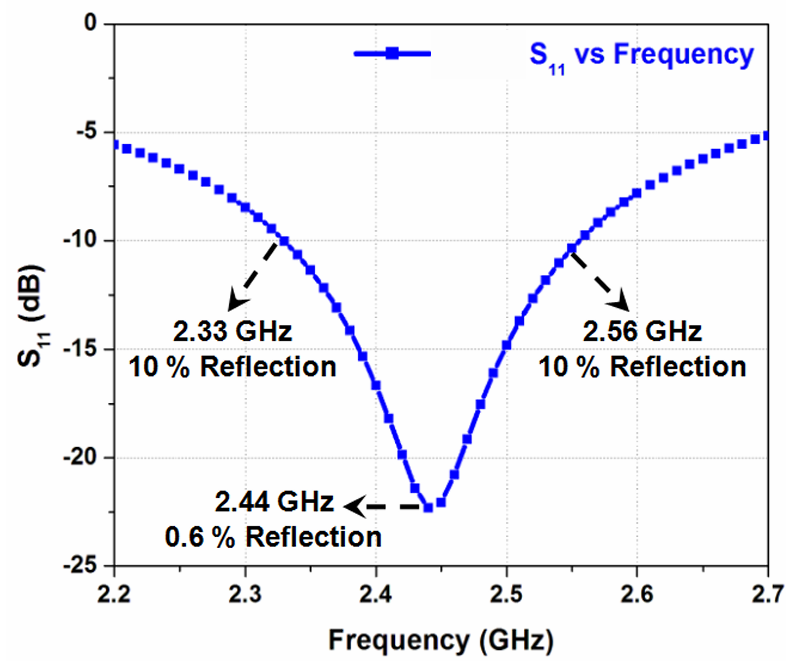
\includegraphics[width=0.5\textwidth]{figures/bandwidth.png}
                \caption{Bandwidth}
                \label{fig:bandwidth}
            \end{figure}

            \autoref{fig:bandwidth} cho thấy return loss lớn hơn 10 dB,
            từ 2.33 GHz đến 2.55 GHz, do đó băng thông là khoảng 200 MHz.
            Băng thông rộng hơn được ưu tiên hơn, vì nó giảm thiểu tác động của
            sự mất điều chỉnh do sự ảnh hưởng của môi trường xung quanh antenna.\par

        \subsection{Radiation efficiency (Hiệu suất bức xạ)}
            Một phần công suất không bị phản xạ bị tiêu tán dưới dạng nhiệt
            hoặc tổn thất nhiệt trong antenna, do chất điện môi trong chất nền FR4 và trên dây dẫn đồng.\par    

        \subsection{Radiation pattern}
            Radiation pattern chỉ ra tính chất định hướng của bức xạ,
            tức là hướng nào có nhiều bức xạ hơn, hướng nào có ít bức xạ hơn.\par
            
            Một antenna lưỡng cực đẳng hướng bức xạ đồng đều theo mọi hướng
            trên mặt phẳng vuông góc với trục antenna. Tuy nhiên, hầu hết các antenna
            không lý tưởng, \autoref{fig:radiation_pattern} cho thấy cường độ trường RF
            không hoàn toàn là hình tròn, vì antenna là không đẳng hướng.\par
            \begin{figure}[h]
                \centering
                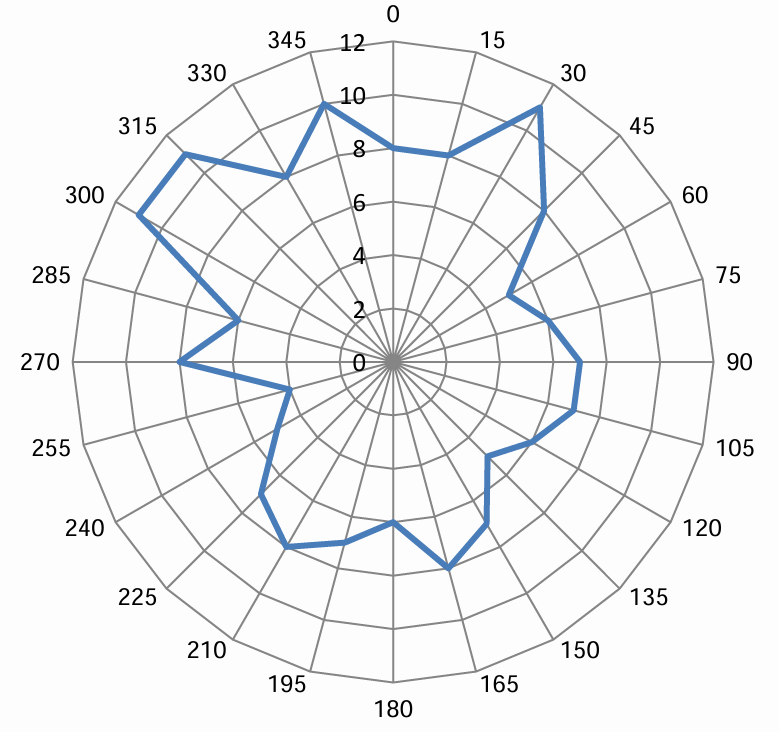
\includegraphics[width=0.3\textwidth]{figures/radiation_pattern.png}
                \caption{Radiation Pattern}
                \label{fig:radiation_pattern}
            \end{figure}

        \subsection{Gain (Độ lợi)}
            Độ lợi biểu thị bức xạ theo hướng cụ thể so với antenna đẳng hướng.
            Điều này được thể hiện theo đơn vị dBi (decibel isotropic) - mực độ mạnh
            của trường bức xạ so với antenna đẳng hướng lý tưởng.\par

    \section{Antennas for Cypress PRoC/PSoC BLE}